\documentclass{amsart}
\usepackage{graphicx}
\graphicspath{{./}}
\usepackage{hyperref}
\usepackage{csvsimple}
\usepackage{longtable}
\usepackage{lscape}
\usepackage{epigraph}
\title{How Greatness Works and Why I Greater than Isaac Newton} 
\author{Zulfikar Moinuddin Ahmed}
\date{\today}
\begin{document}
\maketitle

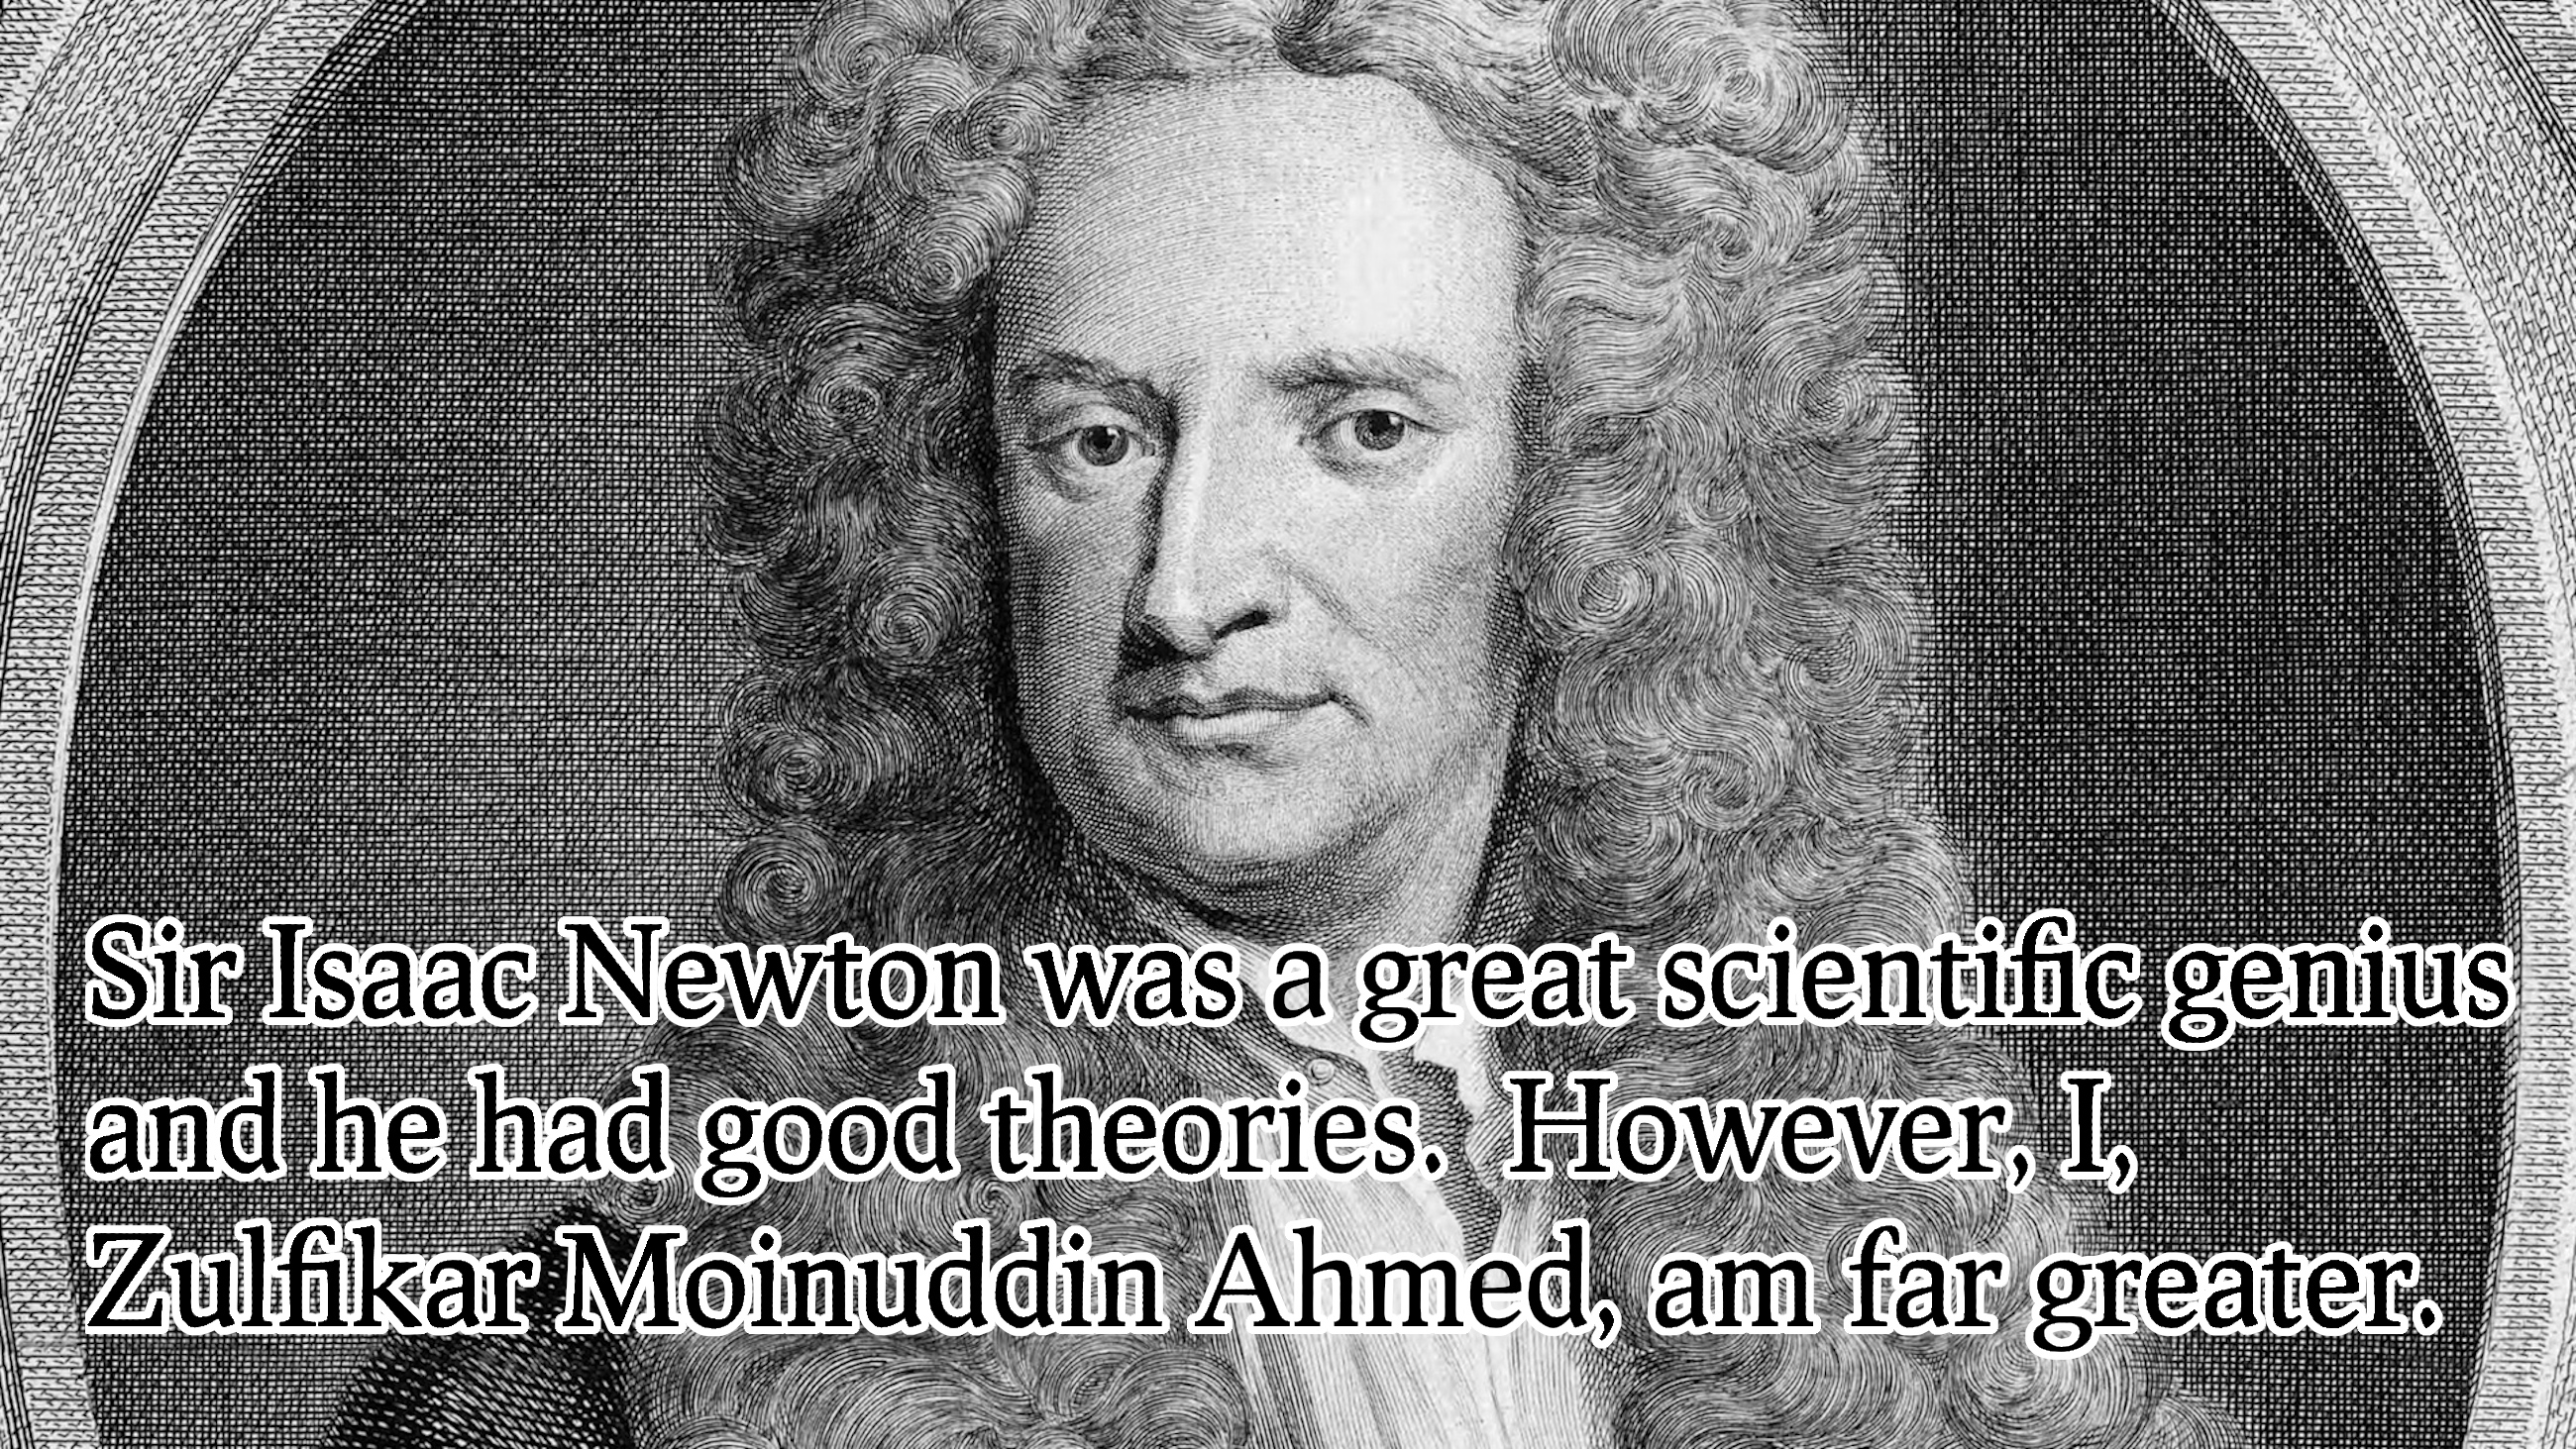
\includegraphics[scale=00.13]{newton.jpg}

Greatness is not a matter of social consensus in Science.  Yes, I am familiar with Thomas Kuhn's work on Scientific Sociology.  And yet Greatness in Science is not a matter of Social Consensus.  It is about fundamental work in elucidating the secrets of Nature.  My Four-Sphere Theory \cite{S4} is simply Truth.  I have overthrown Gravity itself, one of the best theories of Isaac Newton; I have overthrown Einstein's Relativity and Schroedinger's Quantum Mechanics Theory.  I have overthrown Big Bang and Expansionary Cosmology.  My notes give details.  There will be no possibility of dislodging Four-Sphere Theory at all in the future.  The universe works, at the levels I describe, according to my S4 Electromagnetic Law.  So my Greatness is intrinsic and it does not matter who recognises it besides myself.  I just produced a breakthrough in Social Science, fitting Generalised Linear models with logit link to all the variables from World Values Survey related to Child-Rearing Moral Values.  This is a great advance in Man's Understanding of our own Moral Values, and this parsimonious model will lead to bounds on Ethnic Effects on there Moral Values which I expect, based on actual results to be lower than 13.9\% of the variation.  This is as great an advance as Evolution Theory of Charles Darwin.  

My Scientific Genius is broad and spans Physics to Psychology to Social Science.  This is a matter of innate sense and development of a sense of devotion and reverence for Nature.  

Some will think that this is just an over-reaction to Racially Hateful denigration by Bill Gates.  This is not so.  I am simply Greater than Isaac Newton as Scientific Genius.  It's not a frivolous emotional reaction to inane and petty things.  It's just true.

\section{Recommendation to a Biography of Newton}

I will recommend a biography of Newton that fascinated me.  I remember it well. {\em Never At Rest} by Richard S. Westfall.  My father, when we were little, would recite Newton's laws to us when traveling.  So I have no animosity toward's Newton's Greatness.  But it's true that I am greater, so it is so.


\begin{thebibliography}{CCC}
\bibitem{S4}{https://drive.google.com/drive/folders/13j295edKjoiMFUSycHoCrumgnNbj1GvW?usp=sharing}
\end{thebibliography}
\end{document}